\documentclass[12pt,spanish]{article}
\usepackage[spanish]{babel}
\usepackage{graphicx}
\usepackage{color}
\usepackage{xcolor}
\usepackage{colortbl}
\usepackage{amsthm,thmtools}
\usepackage{dirtytalk}
\usepackage{multirow}
\usepackage{amsmath}
\usepackage{subcaption}
\usepackage{adjustbox}
\usepackage{amsmath}
\usepackage{centernot}
\usepackage{mathtools}
\usepackage{multirow}
\usepackage[hidelinks]{hyperref}
\usepackage{caption}
\usepackage{eurosym} % para el euro
\usepackage{amsthm}
\usepackage{multicol}
\usepackage{float}
\usepackage{amsfonts}
\usepackage{titling}
\usepackage{soul}
\usepackage{listings}
\usepackage{array}
\usepackage{tikz}
\usetikzlibrary{shapes.geometric, arrows, chains, calc,positioning,fit,decorations.pathreplacing}
\usepackage[framemethod=tikz]{mdframed}

\graphicspath{ {../../img/}}
\selectlanguage{spanish}
\usepackage[utf8]{inputenc}
\usepackage{graphicx}
\usepackage[a4paper,left=3cm,right=2cm,top=2.5cm,bottom=2.5cm]{geometry}

\newenvironment{solution}{
	\par
	\textbf{Solución}
	\par
	\begin{center}
}
{
	\end{center}
}

\lstset{
  breaklines=true,
  postbreak=\mbox{\textcolor{red}{$\hookrightarrow$}\space},
}


\title{Servidores Web de Altas Prestaciones}
\setlength{\droptitle}{10em}
\author{Carlos Sánchez Páez}

\makeindex
\begin{document}
\definecolor{light-gray}{gray}{0.95}
\lstset{columns=fullflexible,basicstyle=\ttfamily}
\surroundwithmdframed[
  hidealllines=true,
  backgroundcolor=light-gray,
  innerleftmargin=0pt,
  innertopmargin=0pt,
  innerbottommargin=0pt]{lstlisting}


\begin{titlepage}

 \newlength{\centeroffset}
 \setlength{\centeroffset}{-0.5\oddsidemargin}
 \addtolength{\centeroffset}{0.5\evensidemargin}
 \thispagestyle{empty}

 \noindent\hspace*{\centeroffset}
 \begin{minipage}{\textwidth}

  \centering
  
\includegraphics[width=0.9\textwidth]{logo_ugr.jpg}\\[1.4cm]

  \textsc{ \Large Servidores Web de Altas Prestaciones\\[0.2cm]}
  \textsc{GRADO EN INGENIERÍA INFORMÁTICA}\\[1cm]

  {\Huge\bfseries Instalación de ZEVENET \\}
 \end{minipage}

 \vspace{1.5cm}
 \noindent\hspace*{\centeroffset}
 \begin{minipage}{\textwidth}
  \centering

  \textbf{Autor}\\ {Carlos Sánchez Páez}\\[2.5ex]
  
\includegraphics[width=0.4\textwidth]{etsiit_logo.png}\\[0.1cm]
  \vspace{1.5cm}
  
\includegraphics[width=0.15\textwidth]{atc.jpg}\\[0.1cm]
  \vspace{1cm}
  \textsc{Escuela Técnica Superior de Ingenierías Informática y de Telecomunicación}\\
  \vspace{1cm}
  \textsc{Curso 2019-2020}
 \end{minipage}
\end{titlepage}
\thispagestyle{empty}
\newpage
\tableofcontents{}
\newpage


En esta tarea instalaremos Zevenet en una nueva máquina y la configuraremos como balanceador de carga.

\section{Instalación}
\begin{enumerate}
	\item Descargamos la ISO de Zevenet desde https://github.com/zevenet/zlb/releases
	\item Creamos una máquina virtual, la conectamos a la NAT y a la interfaz Host-only.
	\item Arrancamos desde la ISO descargada.
	\item Elegimos idioma y distribución de teclado.
	\item Cuando se nos pidan, especificamos los siguientes parámetros:
	\begin{itemize}
		\item IP: 192.168.56.105/24
		\item Máscara de red: 255.255.255.0
		\item Gateway y servidor DNS: 192.168.56.1
		\item Nombre del host: M4
		\item Nombre de dominio: servidoresSWAP
		\item Clave de superusuario: Swap1234
		\item Zona horaria: Madrid
	\end{itemize}
	\item Elegimos el particionado guiado usando todo el disco (todos los archivos en una partición) e instalamos GRUB.
	\item Cuando termine la instalación, reiniciamos la máquina y nos logueamos (root/Swap1234).
	\item Configuramos las interfaces de red con \emph{netplan}:
	\begin{lstlisting}
	m4 > nano /etc/netplan/nets.yaml
	\end{lstlisting}
	\begin{lstlisting}
	network:
		version: 2
		renderer: networkd
		ethernets:
			eth0:
				dhcp4: yes
			eth1:
				dhcp4: yes
	\end{lstlisting}
	\begin{lstlisting}
	m4 > netplan apply
	\end{lstlisting}
	\item Accedemos a la GUI desde el navegador del host e iniciamos sesión con las credenciales \emph{root/Swap1234}:
	\begin{lstlisting}
	https://<IP M4>:444
	\end{lstlisting}
	\item Entramos al menú \emph{Local System Load Balancer (LSLB)} y damos a \emph{Create farm}:
	\begin{figure}[H]
		\centering
		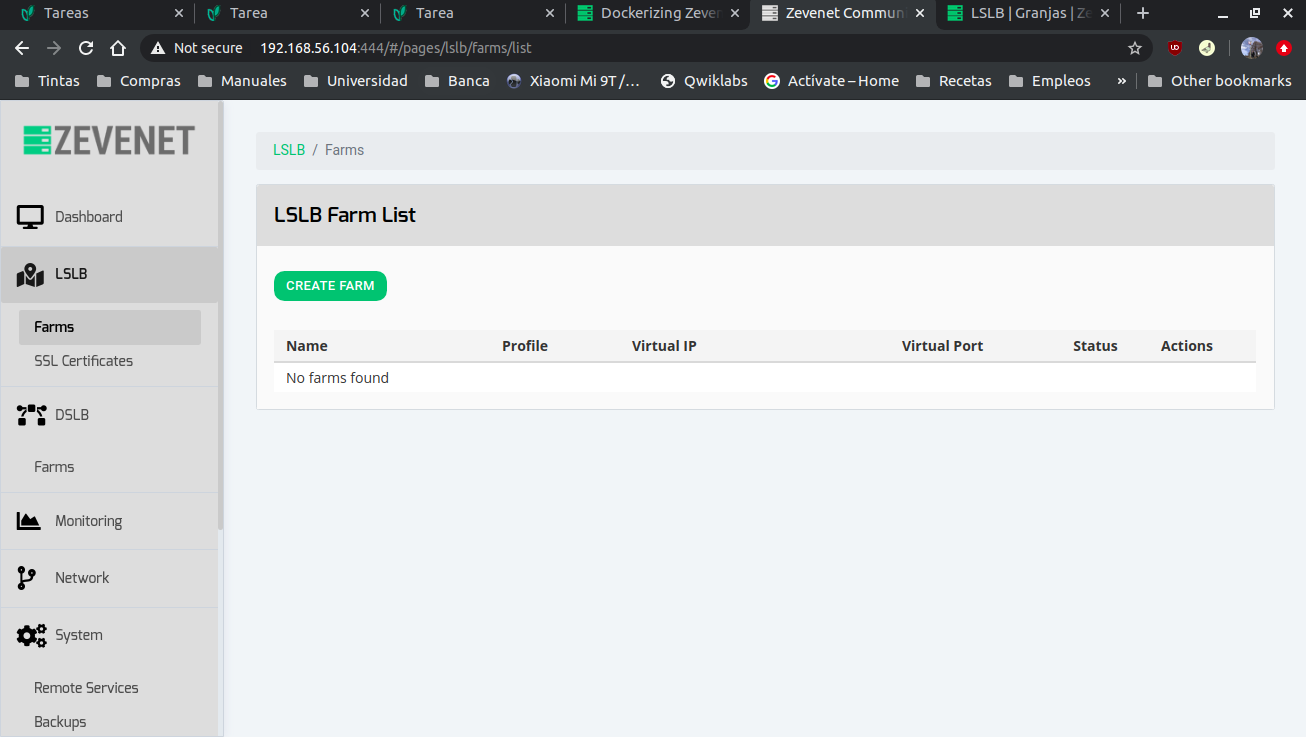
\includegraphics[scale=0.5]{/t4-4/zevenet-1.png}
	\end{figure}
	\item Configuramos los parámetros:
	\begin{figure}[H]
		\centering
		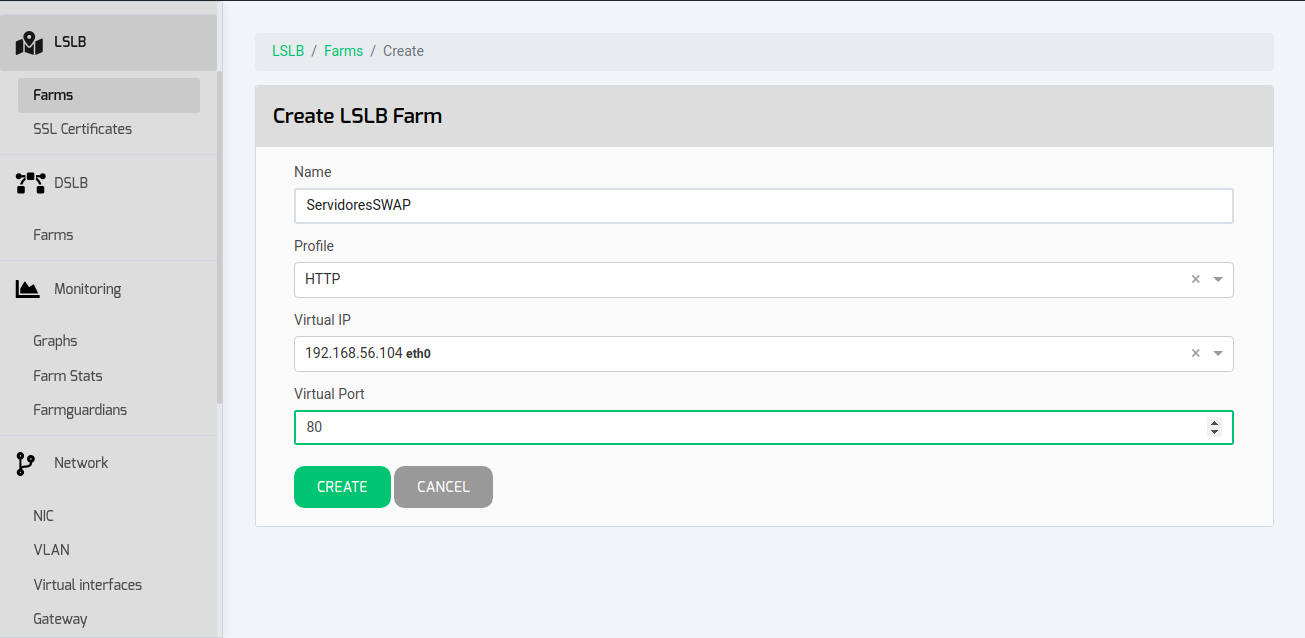
\includegraphics[scale=0.5]{/t4-4/zevenet-2.png}
	\end{figure}
	\item Entramos en los ajustes de la granja:
	\begin{figure}[H]
		\centering
		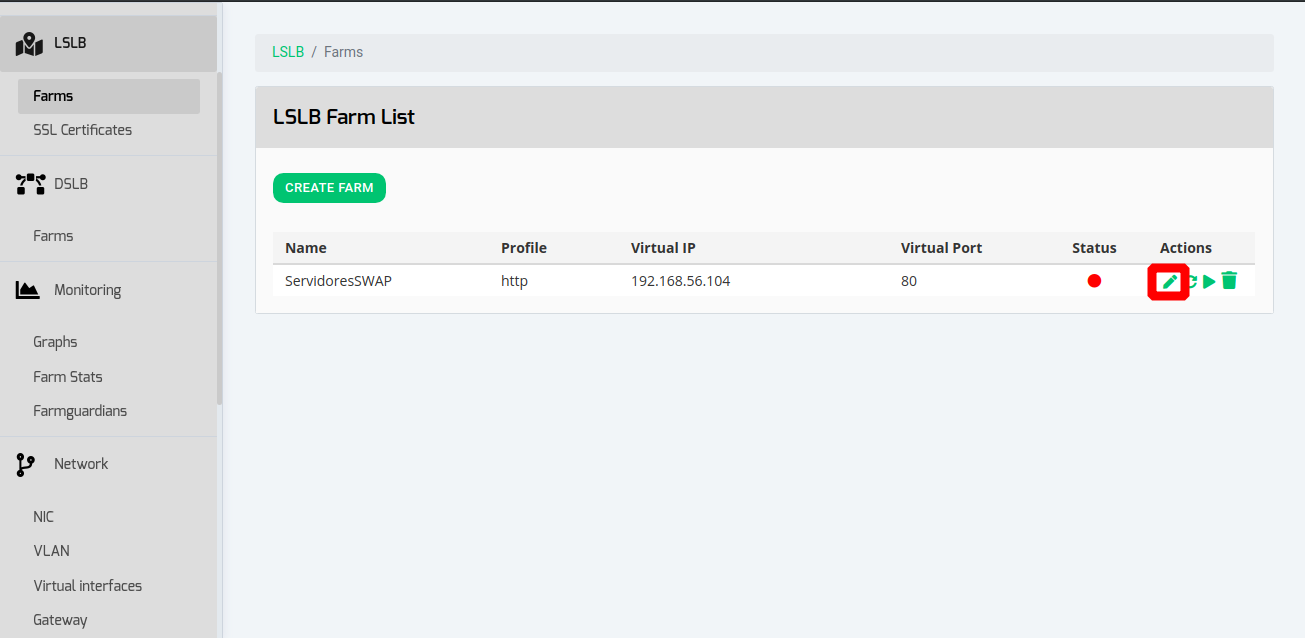
\includegraphics[scale=0.5]{/t4-4/farm-settings.png}
	\end{figure}
	\item Damos de alta un nuevo servicio (\emph{New Service}). Lo llamaremos \emph{ejemplo}.
	\item Añadimos los backends (M1 y M2). Le damos un timeout de 60 segundos y un peso de 1.
	\item Por último, damos en submit y reiniciamos la granja.
	\item Comprobamos su funcionamiento mediante cURL.
	\begin{figure}[H]
		\centering
		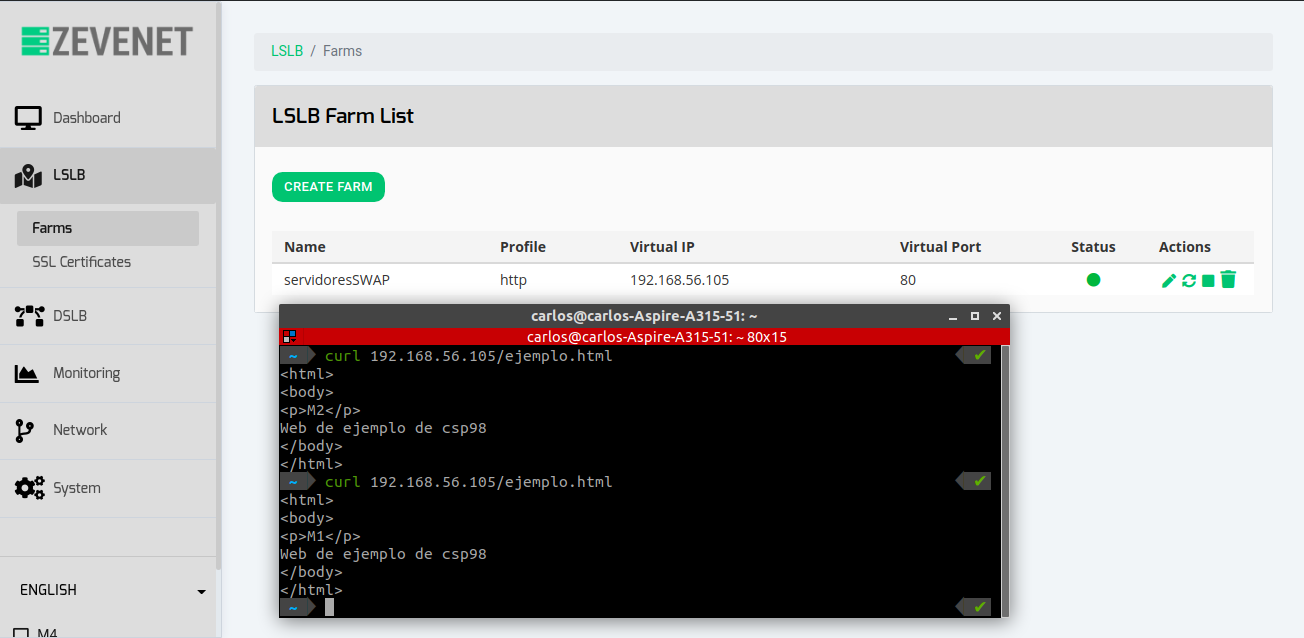
\includegraphics[scale=0.5]{/t4-4/zevenet-ok.png}
	\end{figure}
\end{enumerate}

Este balanceador es mucho más complicado y lento de instalar y configurar que los vistos anteriormente. Sin embargo, ofrece características que los otros no, como un monitor del estado del sistema, GUI de administración, etc.


\end{document}
